%-----------------------------------------------------------------------------------------------------------------------------------------------%
%	The MIT License (MIT)
%
%	Copyright (c) 2019 Jan Küster
%
%	Permission is hereby granted, free of charge, to any person obtaining a copy
%	of this software and associated documentation files (the "Software"), to deal
%	in the Software without restriction, including without limitation the rights
%	to use, copy, modify, merge, publish, distribute, sublicense, and/or sell
%	copies of the Software, and to permit persons to whom the Software is
%	furnished to do so, subject to the following conditions:
%	
%	THE SOFTWARE IS PROVIDED "AS IS", WITHOUT WARRANTY OF ANY KIND, EXPRESS OR
%	IMPLIED, INCLUDING BUT NOT LIMITED TO THE WARRANTIES OF MERCHANTABILITY,
%	FITNESS FOR A PARTICULAR PURPOSE AND NONINFRINGEMENT. IN NO EVENT SHALL THE
%	AUTHORS OR COPYRIGHT HOLDERS BE LIABLE FOR ANY CLAIM, DAMAGES OR OTHER
%	LIABILITY, WHETHER IN AN ACTION OF CONTRACT, TORT OR OTHERWISE, ARISING FROM,
%	OUT OF OR IN CONNECTION WITH THE SOFTWARE OR THE USE OR OTHER DEALINGS IN
%	THE SOFTWARE.
%	
%
%-----------------------------------------------------------------------------------------------------------------------------------------------%


%============================================================================%
%
%	DOCUMENT DEFINITION
%
%============================================================================%

%we use article class because we want to fully customize the page and don't use a cv template
\documentclass[10pt,A4]{article}	


%----------------------------------------------------------------------------------------
%	ENCODING
%----------------------------------------------------------------------------------------

% we use utf8 since we want to build from any machine
\usepackage[utf8]{inputenc}		

%----------------------------------------------------------------------------------------
%	LOGIC
%----------------------------------------------------------------------------------------

% provides \isempty test
\usepackage{xstring, xifthen}
% more control over list spacing
\usepackage{enumitem}

%----------------------------------------------------------------------------------------
%	FONT BASICS
%----------------------------------------------------------------------------------------

% some tex-live fonts - choose your own

%\usepackage[defaultsans]{droidsans}
%\usepackage[default]{comfortaa}
%\usepackage{cmbright}
\usepackage[default]{raleway}
%\usepackage{fetamont}
%\usepackage[default]{gillius}
%\usepackage[light,math]{iwona}
%\usepackage[thin]{roboto} 

% set font default
\renewcommand*\familydefault{\sfdefault} 	
\usepackage[T1]{fontenc}

% more font size definitions
\usepackage{moresize}

%----------------------------------------------------------------------------------------
%	FONT AWESOME ICONS
%---------------------------------------------------------------------------------------- 

% include the fontawesome icon set
\usepackage{fontawesome}

% use to vertically center content
% credits to: http://tex.stackexchange.com/questions/7219/how-to-vertically-center-two-images-next-to-each-other
\newcommand{\vcenteredinclude}[1]{\begingroup
\setbox0=\hbox{\includegraphics{#1}}%
\parbox{\wd0}{\box0}\endgroup}

% use to vertically center content
% credits to: http://tex.stackexchange.com/questions/7219/how-to-vertically-center-two-images-next-to-each-other
\newcommand*{\vcenteredhbox}[1]{\begingroup
\setbox0=\hbox{#1}\parbox{\wd0}{\box0}\endgroup}

% icon shortcut
\newcommand{\icon}[3] { 							
	\makebox(#2, #2){\textcolor{maincol}{\csname fa#1\endcsname}}
}	

% icon with text shortcut
\newcommand{\icontext}[4]{ 						
	\vcenteredhbox{\icon{#1}{#2}{#3}}  \hspace{2pt}  \parbox{0.9\mpwidth}{\textcolor{#4}{#3}}
}

% icon with website url
\newcommand{\iconhref}[5]{ 						
    \vcenteredhbox{\icon{#1}{#2}{#5}}  \hspace{2pt} \href{#4}{\textcolor{#5}{#3}}
}

% icon with email link
\newcommand{\iconemail}[5]{ 						
    \vcenteredhbox{\icon{#1}{#2}{#5}}  \hspace{2pt} \href{mailto:#4}{\textcolor{#5}{#3}}
}

%----------------------------------------------------------------------------------------
%	PAGE LAYOUT  DEFINITIONS
%----------------------------------------------------------------------------------------

% page outer frames (debug-only)
% \usepackage{showframe}		

% we use paracol to display breakable two columns
\usepackage{paracol}

% define page styles using geometry
\usepackage[a4paper]{geometry}

% remove all possible margins
\geometry{top=1cm, bottom=1cm, left=1cm, right=1cm}

\usepackage{fancyhdr}
\pagestyle{empty}

% space between header and content
% \setlength{\headheight}{0pt}

% indentation is zero
\setlength{\parindent}{0mm}

%----------------------------------------------------------------------------------------
%	TABLE /ARRAY DEFINITIONS
%---------------------------------------------------------------------------------------- 

% extended aligning of tabular cells
\usepackage{array}

% custom column right-align with fixed width
% use like p{size} but via x{size}
\newcolumntype{x}[1]{%
>{\raggedleft\hspace{0pt}}p{#1}}%


%----------------------------------------------------------------------------------------
%	GRAPHICS DEFINITIONS
%---------------------------------------------------------------------------------------- 

%for header image
\usepackage{graphicx}

% use this for floating figures
% \usepackage{wrapfig}
% \usepackage{float}
% \floatstyle{boxed} 
% \restylefloat{figure}

%for drawing graphics		
\usepackage{tikz}				
\usetikzlibrary{shapes, backgrounds,mindmap, trees}

%----------------------------------------------------------------------------------------
%	Color DEFINITIONS
%---------------------------------------------------------------------------------------- 
\usepackage{transparent}
\usepackage{color}

% primary color
\definecolor{maincol}{RGB}{ 0, 120, 150 }

% accent color, secondary
% \definecolor{accentcol}{RGB}{ 250, 150, 10 }

% dark color
\definecolor{darkcol}{RGB}{ 70, 70, 70 }

% light color
\definecolor{lightcol}{RGB}{245,245,245}


% Package for links, must be the last package used
\usepackage[hidelinks]{hyperref}

% returns minipage width minus two times \fboxsep
% to keep padding included in width calculations
% can also be used for other boxes / environments
\newcommand{\mpwidth}{\linewidth-\fboxsep-\fboxsep}
	


%============================================================================%
%
%	CV COMMANDS
%
%============================================================================%

%----------------------------------------------------------------------------------------
%	 CV LIST
%----------------------------------------------------------------------------------------

% renders a standard latex list but abstracts away the environment definition (begin/end)
\newcommand{\cvlist}[1] {
	\begin{itemize}[itemsep=0pt]{#1}\end{itemize}
}

%----------------------------------------------------------------------------------------
%	 CV TEXT
%----------------------------------------------------------------------------------------

% base class to wrap any text based stuff here. Renders like a paragraph.
% Allows complex commands to be passed, too.
% param 1: *any
\newcommand{\cvtext}[1] {
	\begin{tabular*}{1\mpwidth}{p{0.98\mpwidth}}
		\parbox{1\mpwidth}{#1}
	\end{tabular*}
}

%----------------------------------------------------------------------------------------
%	CV SECTION
%----------------------------------------------------------------------------------------

% Renders a a CV section headline with a nice underline in main color.
% param 1: section title
\newcommand{\cvsection}[1] {
	\vspace{14pt}
	\cvtext{
		\textbf{\LARGE{\textcolor{darkcol}{\uppercase{#1}}}}\\[-4pt]
		\textcolor{maincol}{ \rule{0.1\textwidth}{2pt} } \\
	}
}

%----------------------------------------------------------------------------------------
%	META SKILL
%----------------------------------------------------------------------------------------

% Renders a progress-bar to indicate a certain skill in percent.
% param 1: name of the skill / tech / etc.
% param 2: level (for example in years)
% param 3: percent, values range from 0 to 1
\newcommand{\cvskill}[3] {
	\begin{tabular*}{1\mpwidth}{p{0.72\mpwidth}  r}
 		\textcolor{black}{\textbf{#1}} & \textcolor{maincol}{#2}\\
	\end{tabular*}%
	
	\hspace{4pt}
	\begin{tikzpicture}[scale=1,rounded corners=2pt,very thin]
		\fill [lightcol] (0,0) rectangle (1\mpwidth, 0.15);
		\fill [maincol] (0,0) rectangle (#3\mpwidth, 0.15);
  	\end{tikzpicture}%
}


%----------------------------------------------------------------------------------------
%	 CV EVENT
%----------------------------------------------------------------------------------------

% Renders a table and a paragraph (cvtext) wrapped in a parbox (to ensure minimum content
% is glued together when a pagebreak appears).
% Additional Information can be passed in text or list form (or other environments).
% the work you did
% param 1: time-frame i.e. Sep 14 - Jan 15 etc.
% param 2:	 event name (job position etc.)
% param 3: Customer, Employer, Industry
% param 4: Short description
% param 5: work done (optional)
% param 6: technologies include (optional)
% param 7: achievements (optional)
\newcommand{\cvevent}[7] {
	
	% we wrap this part in a parbox, so title and description are not separated on a pagebreak
	% if you need more control on page breaks, remove the parbox
	\parbox{\mpwidth}{
		\begin{tabular*}{1\mpwidth}{p{0.72\mpwidth}  r}
	 		\textcolor{black}{\textbf{#2}} & \colorbox{maincol}{\makebox[0.25\mpwidth]{\textcolor{white}{#1}}} \\
			\textcolor{maincol}{\textbf{#3}} & \\
		\end{tabular*}\\[8pt]
	
		\ifthenelse{\isempty{#4}}{}{
			\vspace{-6pt}
			\cvtext{#4}\\
		}
	}

	\ifthenelse{\isempty{#5}}{}{
		\vspace{-8pt}
		{#5}
	}

	\ifthenelse{\isempty{#6}}{}{
		\vspace{0pt}
		\cvtext{\textbf{Technologies:}}\\
		\vspace{-14pt}
		{#6}
	}

	\ifthenelse{\isempty{#7}}{}{
		\vspace{0pt}
		\cvtext{\textbf{Achievements:}}\\
		\vspace{-14pt}
		{#7}
	}
	\vspace{14pt}
}

%----------------------------------------------------------------------------------------
%	 CV META EVENT
%----------------------------------------------------------------------------------------

% Renders a CV event on the sidebar
% param 1: title
% param 2: subtitle (optional)
% param 3: customer, employer, etc,. (optional)
% param 4: info text (optional)
\newcommand{\cvmetaevent}[4] {
	\textcolor{maincol} {\cvtext{\textbf{\begin{flushleft}#1\end{flushleft}}}}

	\ifthenelse{\isempty{#2}}{}{
	\textcolor{darkcol} {\cvtext{\textbf{#2}} }
	}

	\ifthenelse{\isempty{#3}}{}{
		\cvtext{{ \textcolor{darkcol} {#3} }}\\
	}

	\cvtext{#4}\\[14pt]
}

%---------------------------------------------------------------------------------------
%	QR CODE
%----------------------------------------------------------------------------------------

% Renders a qrcode image (centered, relative to the parentwidth)
% param 1: percent width, from 0 to 1
\newcommand{\cvqrcode}[1] {
	\begin{center}
		\includegraphics[width={#1}\mpwidth]{qrcode}
	\end{center}
}


%============================================================================%
%
%
%
%	DOCUMENT CONTENT
%
%
%
%============================================================================%
\begin{document}
\columnratio{0.31}
\setlength{\columnsep}{2.2em}
\setlength{\columnseprule}{4pt}
\colseprulecolor{lightcol}
\begin{paracol}{2}
\begin{leftcolumn}
%---------------------------------------------------------------------------------------
%	META IMAGE
%----------------------------------------------------------------------------------------
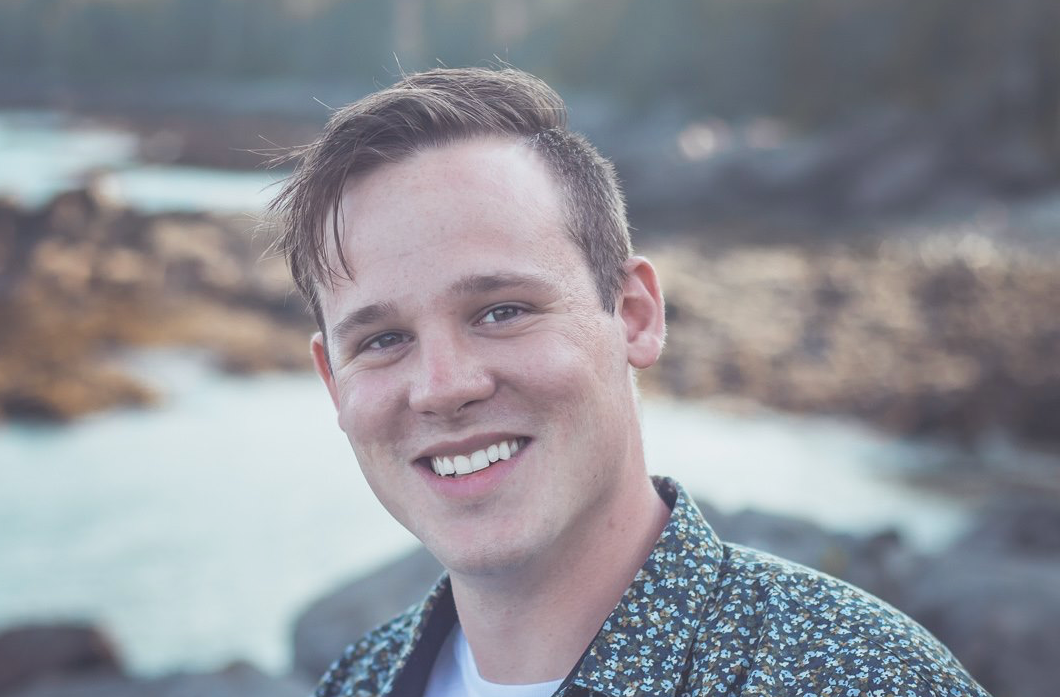
\includegraphics[width=\linewidth]{headshot.png}	%trimming relative to image size

%---------------------------------------------------------------------------------------
%	META SKILLS
%----------------------------------------------------------------------------------------
\cvsection{SKILLS}

\cvskill{Python} {3+ yrs} {1} \\[-2pt]

\cvskill{Linux} {3+ yrs} {1} \\[-2pt]

\cvskill{Git} {3+ yrs} {1} \\[-2pt]

\cvskill{Microcontrollers} {2+ yrs} {0.8} \\[-2pt]

\cvskill{C++} {2+ yrs} {0.9} \\[-2pt]

\cvskill{C} {2 yrs} {0.6} \\[-2pt]

%\cvskill{Firmware} {1+ yrs} {0.5} \\[-2pt]

\vfill\null
%---------------------------------------------------------------------------------------
%	EDUCATION
%----------------------------------------------------------------------------------------
\cvsection{EDUCATION}

\vspace{-10pt}

\cvmetaevent
{Texas A\&M University}
{2012 - 2016, 3.6 GPA}
{B.Sc. Electrical Engineering.}
{Senior Design: \\
%A Framework for Near-Realtime Signal of Interest Identification and Reconstruction for Audio Augmented Reality Applications
Realtime Audio Signal Identification and Reconstruction
}

\vfill\null
%%---------------------------------------------------------------------------------------
%%	MISC	
%%----------------------------------------------------------------------------------------
%\cvsection{PATENTS}
%
%	\icontext{FileTextO}{12}{Device Aware Network Communication Management}{black}\\[6pt]
%
%\vfill\null
%---------------------------------------------------------------------------------------
%	CONTACT
%----------------------------------------------------------------------------------------
\cvsection{CONTACT}
	
\icontext{MapMarker}{12}{Austin, Texas}{black}\\[6pt]
\icontext{MobilePhone}{12}{979 599 8847}{black}\\[6pt]
\iconemail{Envelope}{12}{justindavid.ginn@gmail.com}{justindavid.ginn@gmail.com}{black}\\[6pt]
\iconhref{Github}{12}{https://github.com/jdginn}{https://github.com/jdginn}{black}\\[6pt]
\iconhref{Linkedin}{12}{/justin-ginn}{http://linkedin.com/in/justin-ginn-2429b7126}{black}\\[6pt]

\vfill\null
%\cvqrcode{0.7}

\pagebreak

%---------------------------------------------------------------------------------------
%	SOFT SKILLS
%----------------------------------------------------------------------------------------
\newpage
\cvsection{SOFT SKILLS}

\cvskill{Vision} {} {1} \\[-2pt]

\cvskill{Initiative} {} {1} \\[-2pt]

\cvskill{Innovation} {} {0.9} \\[-2pt]

\cvskill{Leadership} {} {0.8} \\[-2pt]

% Is there a more flavorable word?
\cvskill{Communication} {} {0.8} \\[-2pt]

\vfill

%---------------------------------------------------------------------------------------
%	TOOLS
%----------------------------------------------------------------------------------------
\cvsection{FAVORITE TOOLS}

\icontext{KeyboardO}{12}{you should see my .vimrc}{black}\\[6pt]
\icontext{Search}{12}{ripgrep}{black}\\[6pt]
\icontext{CodeFork}{12}{love a good rebase}{black}\\[6pt]
%\vcenteredhbox{\icon{Linux}{12}{} \icon{Apple}{12}{}{command line junkie}}  \parbox{0.9\mpwidth}
\icontext{Linux}{12}{command line junkie}{black}\\[6pt]
\icontext{Terminal}{12}{mosh is the new ssh}{black}\\[6pt]

\vfill

\cvsection{PHILOSOPHY}

\begin{small}
\icontext{QuoteLeft}{12}{fight "black magic", wherever it is believed in}{black}\\[6pt]
\icontext{QuoteLeft}{12}{fight technical debt at any cost}{black}\\[6pt]
\icontext{QuoteLeft}{12}{architect for greatness, prioritize the minimum viable product}{black}\\[6pt]
\icontext{QuoteLeft}{12}{leverage your effort}{black}\\[6pt]
\icontext{QuoteLeft}{12}{everyone is a leader}{black}\\[6pt]
\end{small}

\vfill

%---------------------------------------------------------------------------------------
%	OUTSIDE THE OFFICE
%----------------------------------------------------------------------------------------
\cvsection{ACTIVITIES}

\icontext{Music}{12}{music production}{black}\\[6pt]

\vfill\null

\end{leftcolumn}
\begin{rightcolumn}
%---------------------------------------------------------------------------------------
%	TITLE  HEADER
%----------------------------------------------------------------------------------------
\fcolorbox{white}{darkcol}{\begin{minipage}[c][3.5cm][c]{1\mpwidth}
	\begin {center}
		\HUGE{ \textbf{ \textcolor{white}{ \uppercase{ Justin Ginn} } } } \\[-24pt]
		\textcolor{white}{ \rule{0.1\textwidth}{1.25pt} } \\[4pt]
		\large{ \textcolor{white} {Hardware Bringup and Verification Engineer} }
	\end {center}
\end{minipage}} \\[14pt]
\vspace{-12pt}

%---------------------------------------------------------------------------------------
%	PROFILE
%----------------------------------------------------------------------------------------
\vfill\null
	\vspace{-10pt}
\cvsection{PROFILE}

\cvtext{
	% Consider fitting more into this first sentence, less jumpy sentence-paragraphs
	% TODO: do I want periods or no periods?
	Proven Computer Engineer with a passion for architecting systems and methodologies to allow teams to reach their full potential.\\

	I am intensely curious and self-motivated, and thrive on learning new skills as I apply them to the challenges I am solving.
	I seek out opporunities to apply vision, innovate,  and develop new methodologies to improve business processes and outcomes.\\

	I am a philosophical programmer who loves writing whitepapers to accompany the systems I deliver.
	Over the course of my career I have discovered a growing interest in software design, especially pertaining to how good software design creates better hardware.
}

%---------------------------------------------------------------------------------------
%	WORK EXPERIENCE
%----------------------------------------------------------------------------------------
\vfill\null
\cvsection{WORK EXPERIENCE}

\cvevent
	% TODO: do I want periods or no periods?
	{Oct 18 - Present}
	{Microcontroller Assisted Test Lead}
	{IBM}
	{
		Spearheaded test solution \textbf{leveraging firmware code in manufacturing test }to match test to field conditions, improving quality\\
	}
	{\cvlist{
		\item Owned \textbf{boot sequence} for Power10 used in manufacturing, bringup, and burn-in
		\item Drove \textbf{presilicon verification} of test functionality, virtual bringup for firmware
		\item Interfaced with firmware, verification, design, and manufacturing teams to support firmware code at manufacturing test
		\item Trained new hires and educated stakeholder teams in Microcontroller Assisted Test strategy
	}}
	{\cvlist {
		\item \textbf{Architected Python API} to interface with embedded microcontrollers using firmware code written in \textbf{C++}, low level \textbf{C}, and \textbf{assembly language}
		\item Developed interface between embedded microcontrollers and Automatic Test Equipment using Python to comprehend \textbf{ELF} and \textbf{DWARF} binary formats
		\item Managed team's interaction with several large \textbf{Gerrit} repositories
		\item Implemented test-specific content in firmware repositories, including custom \textbf{make} and \textbf{linker} infrastructures
	}}
	{\cvlist{
		\item \textbf{IBM Outsanding Technical Achievement Award for Innovation}, awarded for Microcontroller Assisted Test
		\item Reduced test-sector boot time by \textbf{70\%} generation-over-generation
		\item First-time-right bringup using Microcontroller Assisted Test strategy
	}}

\pagebreak

\vfill\null
\cvevent
	{Oct 17 - Oct 18}
	{Design For Test Engineer}
	{IBM}
	{Functional Exercisers Owner for manufacturing test}
	{\cvlist{
	\item Created register-level test sequences to power on, configure, load, and execute \textbf{functional workloads} on the processor
		\item Delivered test patterns for \textbf{Teradyne Ultraflex} and J973 ATE platforms
		\item Supported voltage droop mitigation sensor testing and calibration for use in \textbf{Power Management}
		\item Interfaced with circuit and system characterization teams to support test to real-world correlation
	}}
	{\cvlist {
		\item Automation using \textbf{Perl}, \textbf{Python} and shell scripting in \textbf{Linux}
	}}
	{}
	{}

\vfill\null
\cvevent
	{Jan 17 - Oct 17}
	{Processor Failure Analysis Engineer}
	{IBM}
	{Root-caused manufacturing test escapes to improve test coverage and Shipped Product Quality Level for Power9}
	{\cvlist{
		\item Delivered enhanced manufacturing test patterns to eliminate a category of test escapes
		\item Identified opportunities for manufacturing test improvements based on \textbf{System Level Test} feedback
		\item Assisted with array and functional coverage improvements to support Power9 bringup and General Announcement
	}}
	{}
	{}

\vfill\null
\cvevent
	{May 16 - Aug 16}
	{Product Engineering Intern}
	{NXP}
	{Created utility to identify and discard unprofitable die locations, improving gross margin, yield, and reliability}
	{\cvlist{
		\item{Engaged with Product and Test Engineering teams to understand cost implications of yields at each test insertion}
%		\item{Processed die-level yield information from multiple databases to automate profitability impact measurements}
%			\item{Delivered graphical user interface for widepsread deployment}
	}}
	{\cvlist{
		\item Scripting in \textbf{JMP} for data analysis and profitability calculation
	}}
	{\cvlist{
		\item Awarded for \textbf{best intern presentation} in Microcontrollers Division, 2016
	}}

\vfill\null
\cvevent
	{May 15 - Jul 15}
	{Test Engineering Intern}
	{National Instruments}
	{Developed a suite of tools to automatically configure network ports and device configuration in test stations}
	{\cvlist{
	\item Designed in-house replacement for LED test equipment, saving a potential \textbf{\$35,000 over 3 years}
	}}
	{\cvlist{
		\item{Used \textbf{Labview} and shell scripting for automation utility}
	}}
	{}

\vfill\null
\cvsection{PATENTS AND PUBLICATIONS}

	\icontext{FileTextO}{12}{Device Aware Network Communication Management}{black}\\[6pt]
	\icontext{FileTextO}{12}{A Framework for Near-Realtime Signal of Interest Identification and Reconstruction for Audio Augmented Reality Applications}{black}\\[6pt]

\vfill\null
\end{rightcolumn}
%\clearpage
\end{paracol}
\end{document}

